\RequirePackage[l2tabu, orthodox]{nag} 					% Checks for obsolete syntax and package % Layout
\documentclass[11pt,a4paper,oneside]{article}
%% font

\usepackage{MnSymbol}
\usepackage[mathlf,textlf]{MinionPro}
\usepackage[T1]{fontenc}
\usepackage{textcomp}
\usepackage{enumitem}
\usepackage{undertilde}

%% Author
\def\myaffiliation{University of Copenhagen}
\def\myauthor{Rud Faden}
\def\myemail{rud.faden@econ.ku.dk}
\def\mytitle{Physician Information Acquisition In a Dynamic Setting}
\def\mykeywords{Information aggregation, physician,}

%% packages
\usepackage{faden}
\pgfplotsset{compat=1.9}
\usetikzlibrary{decorations.pathreplacing}
\graphicspath{{../fig/}}
\usepackage{commath}

%% biblatex path
% \addbibresource{Remote.bib}
\addbibresource{Remote.bib}

% Author and title
\title{\mytitle}
\author{
{\myauthor} \\
\textit{\small \myaffiliation} \\
\small{\texttt{\href{\myemail}{\myemail}}}
}
\date{\today} % no date

% Custom commands

\begin{document}

\maketitle

%%--------------------------------------------------------------------------
%% Abstract
%%--------------------------------------------------------------------------
\begin{abstract}
In this project, I examine provider and patient demand for information in a dynamic model where the diagnostic precision is assumed to be related to physician effort, and effort is non-contractible. In each period where the patient and physician interact, the physician gathers information about the patient, and the diagnostic precision is increased. Therefore, optimal physician effort decreases as the physician and patient tie increases. As the physician is unobserved, the insurer compensates the physician by the average effort in the physician population and physician will not provide an optimal level of diagnostic precision in the in the first encounters with a new patient. Therefore the switching cost of the patient increases as the tie with the physician lengthens. This model explains (i) why the cost is negatively related with patient, physician ties and (ii) also introduces the concept of an ``information trap'', where competition is deceasing in the patient physician tie as switching cost increases. Increases.
\end{abstract}
%%--------------------------------------------------------------------------
%% Introduction
%%--------------------------------------------------------------------------
\section{Introduction}
It is a popular view among doctors that long term relationship between doctor and patient is a vital to good primary health care and promote patient satisfaction, and cost-effectiveness. Long term relationships are thought to increase in value because
\begin{quotation}
the practitioners come to know patients over time, and patients come to know the practitioners. The benefits of this knowledge [can] be expected to accrue in a variety of ways. For example, patients should make fewer visits be- cause many problems can be managed on the phone. Fewer hospitalizations should also result, since practitioners are more likely to be able to ascertain whether or not the problem [can] be managed at home \parencite[p. 41--42]{Starfield1992}.
\end{quotation}
and
\begin{quotation}
it \ldots \ takes time for physicians to understand and empathize with patients' values and feelings and to be able to help patients identify and utilize health care services that are appropriate for their condition and life situation\ldots Decisions to adopt healthy habits, to stop smoking to spare a child from passive smoke \ldots are more likely to be made if recommended by a trusted physician in the context of an ongoing relationship \parencite[p. 324--235]{Emanuel1995}.\todo{find more recent quotation}
\end{quotation}
This has to some degree been backed by empirical evidence. Using insurance data \textcite{Weiss1996} find that long-term relations are associated with more preventive care, less hospitalization, and lower costs. However \citeauthor{Weiss1996} does not attempt to separate matching effects from the patient tie effect, which makes the results hard to interpret. In another study on the physician knowledge about his patient,   \textcite{Hjortdahl1991}  finds that physicians with more knowledge about a patient is less likely to order lab tests, more likely to adopt a ``wait-and-see'' approach, and more likely to prescribe drugs and refer patients to specialists.

Despite this evidence, models that incorporate physician knowledge about their patients are scares, and no models exists which describes how physician knowledge is obtained.

In my model, information about a patient is seen as an economics good, which can be produced at a cost \(c\) by the physician. Further it attempts to describe the process of how information is accumulated by the physician and how this may both decrease cost and competition among physicians at the same time.

Very general models of learning have been developed by \textcite{Grossman1977}. However such a model quickly becomes very complex and as a results applications are not easy. Instead I limit myself to a class of monotone decision problems, which greatly simplifies the analysis.
%%--------------------------------------------------------------------------
%% Section: The Patients Utility}
%%--------------------------------------------------------------------------

\section{The Patients Utility}

Following \citet{Rochaix1989}, the patient has a utility function
\[
	U = u(t,s):\, T\times S\longrightarrow\mathbb{R}
\]
where \(t\) is treatment, \(s\) is disease variable classified by its severity of illness, where both \(t\) and \(s\) traverse a real line. It is assumed that the utility function has both increasing and decreasing parts to capture the negative effects of both under and over treatment. It is further assumed that the dis-utility of moving away from the optimum is increasing in \(s\)  such that the patient is more \emph{risk-sensitive} for higher values of \(s\)

%========== DEFINITION: Risk-sensitivity ==========%
\begin{definition}\label{def:risk-sensitivity}
Assuming that the decision problem has a unique solution \(t^{*}(s)\)  and for \(s'>s\),  \(u(t^{*}(s),s)=u(t^{*}(s'),s')\). Then for \(t^{*}(s)>t_{1}\), \(t^{*}(s')>t_{2}\),  \(t_{2}\ge t_{1}\), and \(t^{*}(s')-t_{2}=t^{*}(s)-t_{1}=\Delta t\) the \emph{risk-sensitivity} is monotonically increasing in \(s\)  if
\[
	0\le u(t^{*}(s),s)-u(t_{1},s)\le u(t^{*}(s'),s')-u(t_{2},s')\label{eq:risk-sensitivity}
\]
for all \(s\) and \(t\)  and I write that \(u(t_{1},s)\preceq u(t_{2},s')\)
\end{definition}
%==================================================%

The notion of \emph{risk-sensitivity} is illustrated in \cref{fig:The-patients-utility}.

%========== THEOREM: Single crossing property ==========%
\begin{theorem}\label{thm:single-crossing}
If the risk sensitivity is increasing in \(s\)  then for \(s'>s\), \(u(t,s)\) has a single crossing property in \((s,t)\)
\end{theorem}
%==================================================%

%========== PROF - crossing property ==========%
\begin{proof}
Let \(t'=t^{*}(s')\) and \(t=t^{*}(s)\). Given \cref{def:risk-sensitivity}, it is clear that \(t'\ge t_{2}>t\ge t_{1}\). Therefore I can rewrite \cref{eq:risk-sensitivity} as
\begin{align}
  u(t',s')-u(t_{2},s')\ge u(t,s)-u(t_{1},s)\ge0\label{eq:increasing-differences}
\end{align}
\cref{eq:increasing-differences} clearly have increasing differences in \(s\) and thereby satisfies the single crossing property.
\end{proof}
%==================================================%

The intuition behind \cref{thm:single-crossing}, is that the marginal change \(u(t',\cdot)-u(t,\cdot)\) is larger, when \(s\) is larger. When \(u(t,s)\) is differentiable and concave as in \cref{fig:The-patients-utility}, one might note \(\partial u(t,s)/\partial t\ge0\) for \(t\le t^{*}(s)\) and that for \(\partial u(t,s)/\partial t\le0\) for \(t\ge t^{*}(s)\). Thereby \(\partial u(t,s')/\partial t>\partial u(t,s)/\partial t\) for \(t\le t^{*}(s)\) and \(\partial u(t,s')/\partial t<\partial u(t,s)/\partial t\) for \(t\ge t^{*}(s)\). One might also note that \(\partial u(t,s')/\partial t\) crosses \(\partial u(t,s)/\partial t\) at most once, and only from below.

%========== FIGURE: Utility and single-crossing ==========%
\begin{figure}
     \centering
    \begin{subfigure}[b]{0.49\textwidth}
		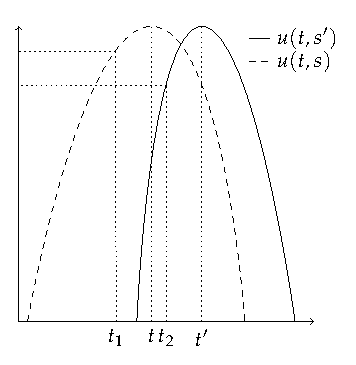
\includegraphics[width=\textwidth]{patient-utility.pdf}
	\end{subfigure}
    \begin{subfigure}[b]{0.49\textwidth}
		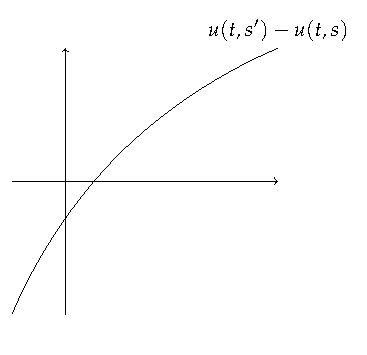
\includegraphics[width=\textwidth]{single-crossing-property.pdf}
	\end{subfigure}
\caption{\label{fig:The-patients-utility}The patients utility functions. If for the same change in \(t\) the loss in utility is smaller for \(s\) than for \(s'\)  when \(s<s'\)  then I says that risk sensitivity is increasing in \(s\) }
\end{figure}
%=======================================================%

%========== PROPOSITION: Single-crossing property ==========%
\begin{proposition}
Given that \(u(t',s)-u(t,s)\) has a single crossing propositionerty in \(s\) and that both \(S\) and \(T\) are well ordered sets (in the strong set order)\footnote{If \(X' \geq X\) in the strong set order, then \(\max (x',x)\in X'\) and \(\min (x',x)\in X\). E.g.\ \([2,5]\geq[0,3]\) in the strong set order, while \(\{2,5\} \) and \(\{0,3\}\) is not. \\
	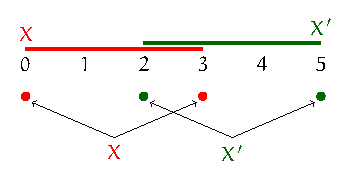
\includegraphics[width=0.4\textwidth]{strong-set-order.pdf}
}, then
\[
	t^{*}(s)=\argmax_{s\in S}u(t,s)\label{eq:increasing-solution}
\]
is increasing in \(s\).\footnote{It should be noted that the assumption of quasi-supermodularity is not needed as the choice space is well ordered (e.i.\ a chain).}
\end{proposition}

\begin{proof}
As both \(T\) and \(S\) are real lines, then it follows trivially that they are well ordered. For the rest of the proof see \textcite{Milgrom1994} or \cref{app:topiks-proof}
\end{proof}
%===========================================%

%========== EXAMPLE: Single-crossing ==========%
\begin{example}
A function with the properties defined in \cref{thm:single-crossing} and \cref{eq:risk-sensitivity} and have the form as in \cref{fig:The-patients-utility} is
\[
	u(t,s) = c-s{(s-t)}^{2}\label{eq:utility-example}
\]
where \(t,s\in\mathbb{R}^{+}\). Assuming that \cref{eq:utility-example} is continuous and twice differential in \(t,s\)  the derivative \(\partial^{2}u(t,s)\big/\partial t\partial s=2s^{2}\ge0\) and \cref{eq:utility-example} has increasing differences and thereby also a single crossing property in \((t,s)\)
\end{example}
%============================================%

%%--------------------------------------------------------------------------
%% Section: Uncertainty with perfect agency
%%--------------------------------------------------------------------------

\section{Uncertainty with perfect agency}

In reality however, \(s\) is never observed. The level of severity for the patients is a random variable represented by \(S\)  characterized by a subjective CDF.\@ \(F(s)\)  with density \(f(s)\)  where \(s\) is a realization of \(S\). The expected value of choosing an admissible treatment intensity \(t\) is given by
\[
	U(t,S)=E[u(t,s)]=\max_{t}\int_{S}u(t,s)\dif F(s)\label{eq:expected-utility-prior}
\]
It is however possible to acquire costly information about \(s\) through medical diagnostics and physician effort. However, for two experiment \(X,Y\) on \(S\)  it is not a priori certain that one experiment \(X\) is necessary more \emph{informative} about \(s\) than the experiment \(Y\)  where \emph{informative} is to be understood in the way the posterior decision induced by the experiment \(X\) insures greater expected utility than the decision induced by the experiment \(Y\). Therefore we must introduce an order of information.

%%--------------------------------------------------------------------------
%% Section: Information ordering
%%--------------------------------------------------------------------------

\subsection{Information ordering}

%========== DEFINITION: affiliation ==========%
\begin{definition}\label{def:afflilation} \parencite{Milgrom1982a}
For a family of density functions, let \(x\lor s\) denote the component wise maximum and \(x\land s\) the component wise minimum. Then \(x\) and \(s\) are affiliated if for all \(s\) and \(x\)
\[
	f(s\lor x)\, f(s\land x)\ge f(s)\, f(x)
\]
\end{definition}
%=============================================%

Affiliation of two random variables are equivalent to the monotone likelihood ratio property, and the intuition behind \cref{def:afflilation} is that higher signal realization of \(x\) makes the probability that \(s\) is large, higher. Similarly small signal realization of \(x\) makes the probability of a small \(s\) more likely.\footnote{See \cref{app:affiliation} for more details}

\textcite{Athey2002}  shows that solution given in \cref{eq:increasing-solution} is robust to uncertainty, such that
\[
	t^*(x)=\argmax_{x\in X}\int_Su(t,s)\dif G^\eta(s\mid x)
\]
is increasing in \(x\)  whenever \(x\) and \(s\) are affiliated.\footnote{Note that here we, unlike in \cref{thm:informative}, consider the problem of deciding a treatment \(t\) before the state \(s\) is know, but \emph{after} observing the signal \(x\) }

%========== DEFINITION: Accuracy ==========%
\begin{definition}\label{def:accuracy}
\parencite{Persico2000} Given two signals (experiments) \(X^{\eta}\) and \(X^{\eta'}\),  \(X^{\eta'}\) is more accurate than \(X^{\eta}\) if
\begin{align}
    	T_{\eta,s}(x)=F^{\eta'^{-1}}(F^{\eta}(x\mid s)\mid s)\label{eq:acuracy tranformation}
\end{align}
is non decreasing in \(s\) for all \(x\).\footnote{Note that \cref{eq:acuracy tranformation} can also be written as \(F^{\eta'}(T_{\eta,s}(x)\mid s)=F^{\eta}(x\mid s)\) which implies that \(T_{\eta,s}(x)\), solves \(f^{\eta'}(x\mid s)=f^\eta(T^{-1}(y)\mid s)T'^{-1}(y)\)} Let \(E\) be a real line. A family of signals \(\left \{ X^{\eta}\right \} _{\eta\in E}\), with support \(X:=\bigcup_{x\in E}X^\eta\), is accuracy ordered (A-ordered) if a signal with higher index is more accurate than a signal with lower index.
\end{definition}
%================================================%

To understand the concept of accuracy, it can be noted that
\[
	T_{\eta,s}(X^{\eta}\mid s)\sim X^{\eta'}\mid s
\]
Thus a more accurate signal can be obtained from a less accurate signal, by the transformation \(T_{\eta,s}(X)\)  For a better understanding of the accuracy concept, see \cref{ex:t-transformation-1,ex:t-transformation-2}.

%========== EXAMPLE: T-transformation 1 ==========%
\begin{example}\label{ex:t-transformation-1}
Let  \(\eta\in[0,\infty)\) and let \(S\) be distributed according to any CDF and let \(X_{\eta}\) be uniformly distributed on \([s-1/\eta,s+1/\eta]\) and let \(f^\eta(x\mid s)=\eta\big /2\) on \(X^\eta\). Then for \(\eta'>\eta\)
\[
	\frac{\eta'}{2}=\frac{\eta}{2}\left(T_{\eta,s}^{-1}\right)'(x)\Leftrightarrow T_{\eta,s}(x)=\frac{\eta}{\eta'}(x-s)+s
\]
To see why, note that

\begin{align*}
	T^{-1}_{\eta,s}(y)               &=\frac{\eta'}{\eta}(y-s)+s \Rightarrow \\
	\left(T^{-1}_{\eta,s}\right)'(y) &=\frac{\eta'}{\eta}
\end{align*}

\begin{figure}
	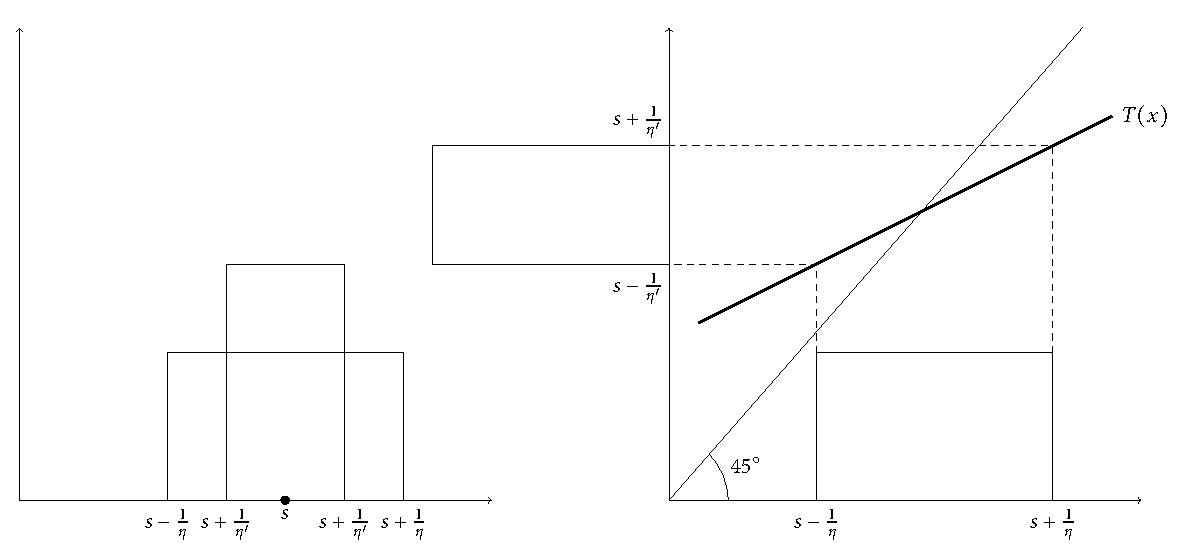
\includegraphics[width=\textwidth]{t-transformation.pdf}
	\caption{\label{fig:t-transformation}The \(T_{\eta,s}(x)\) transformation}
\end{figure}

Further, one might also note that \(T_{\eta,s}(x)\) is an increasing function by taking the derivative
\[
	\frac{\partial^2}{\partial \eta'\partial s}T_{\eta,s}(x)=\frac{\eta}{\eta'^2}>0
\]
Thus, \(T_{\eta,s}(x)\) transforms \(X^{\eta}\) into \(X^{\eta'}\) when \(T_{\eta,s}(x)\) is increasing~\citep{Persico1996}.

From \cref{fig:t-transformation}, the ting to note is that \(T_{\eta,s}(x)\) has a slope less than 1 and crosses the \(45^\circ\) line at \(s\). This means that \(T_{\eta,s}(x)\) contracts mass around \(s\). Further, observe that \(T_{\eta,s}(x)\) is a straight line passing through \((s,s)\). Thus increasing \(s\) to \(s'\) will course \(T_{\eta,s}(x)\) to shift up, so the line passes through \((s',s')\). Hence the notation of ``more accurate signal'' can be interpreted as one signal \(X^{\eta'}\) being more correlated with the random state \(s\) than another signal \(X^\eta\), and the function \(T_{\eta,s}(x)\) imposes this additional correlation.
\end{example}
%=======================================================%

An illustrative example can also be given by applying \cref{eq:acuracy tranformation} to hypothesis testing.

%========== EXAMPLE: T-transformation 2==========%
\begin{example}\label{ex:t-transformation-2}
Consider the case where \(s\) can take two values \(s_{1}<s_{2}\). Let \(X^{\eta}\) be a information structure affiliated with \(S\). The optimal test based on \(X^{\eta}\) is given by the rejection region \(X^{\eta}>x^{*}\)  such that \(s_{1}\) is rejected in favor of \(s_{2}\) when \(X^{\eta}>x^{*}\). The probability of a type I error is then \(\mathbb{P}(X^{\eta}\le x^{*})=F(x^{*}\mid s_{2})\) and the probability of a type II error is \(1-F(x^{*}\mid s_{1})\). Now given that \(X^{\eta'}\) is more accurate than \(X^{\eta}\) is is possible to design a test with the same probability of type I error, by choosing \(x^{**}\) such that \(F(x^{**}\mid s_{2})=F(x^{*}\mid s_{2})\) (e.i. \ accept \(s_{2}\) if \(X^{\eta}\ge x^{**}\) . However, since \(X^{\eta'}\) is more accurate than \(X^{\eta}\)  then \(x^{**}\ge F^{\eta'^{-1}}(F^{\eta}(x\mid s_{1})\mid s_{1})\). As \(x^{**}\) lies on or, to the right of \(x^{*}\) then the test based on \(X^{\eta'}\) is a least as powerful as the test based on \(X^{\eta}\) \citep{Lehmann1988,Persico2000}.\footnote{For a graphical example, see \cref{app:test-power}}
\end{example}
%=====================================================%

%%--------------------------------------------------------------------------
%% Subsection: Demand for information
%%--------------------------------------------------------------------------

\subsection{Demand for information}

Given that we now know, when a test can be considered more informative than another, I can know turn to the problem of informativeness. To use the notation of informativeness I make two assumptions

%==========  ASSUMPTION: needed for proof  ==========%
\begin{assumption}
	The utility function is differential in \(t\) and the optimal solution \(t^*(x)\) is differentiable in in \(\eta\) and \(x\)
\end{assumption}
\begin{assumption}
	For all pairs of signals and states \((s,x)\) the CDF \(G^\eta(s\mid x)\) is differentiable in \(\eta\) on \(E\) and is continuous in \(s\)
\end{assumption}
%====================================================%

%========== THEOREM: informative ==========%
\begin{theorem}\label{thm:informative}
\parencite{Persico2000}
Suppose that \(X^{\eta}\) and \(X^{\eta'}\) are affiliated with \(S\) and that \(\left \{X^{\eta}\right \} _{\eta\in E}\) is A-ordered, such that \(X^{\eta'}\) is more accurate than \(X^{\eta}\). Then for all utility functions with a single crossing property, \(X^{\eta'}\) is more informative than \(X^{\eta}\)
\end{theorem}
% the real important fact here is that u is monotonically increasing in s
\begin{proof}
See \citet{Lehmann1988} section 4 and \citet{Karlin1956} Lemma 3--4 and theorem 1.
\end{proof}
%=============================================%

It follows directly from \cref{thm:informative} that when \(X^{\eta'}\) is more informative than \(X^{\eta}\)  then
\begin{align}
	\label{eq:utility-increasing-information}
	\begin{split}
	\int_{X}\int_{S}u(t,s)\dif G^{\eta'}(s\mid x)\dif F^\eta(x)&\geq \int_{X}\int_{S}u(t,s)\dif G^{\eta}(s\mid x)\dif F^h(x) \Leftrightarrow \\
	U(t,s;\eta')&\geq U(s,t;\eta)
\end{split}
\end{align}

From the above equation, it is clear that the patient will always prefer a more accurate signal to a less accurate signal.

\textcite{Persico2000} goes on to show that when \(u(t,s)\) is risk-sensitive increasing in \(s\), then the marginal value of information
\begin{align}
		MR(\eta)=\frac{\partial}{\partial \eta} \int_{X}\int_{S}u(t,s)\dif G^{\eta}(s\mid x)\dif F^h(x) \label{eq:marginal-value-of-information}
\end{align}


is increasing in \(s\).

From \cref{eq:marginal-value-of-information} it follows straight forward that the optimal level of accuracies defined by
\begin{align}
	MR(\eta)-C(\eta)=0
\end{align}
 is increasing in \(s\), where \(C(\eta)\) is the cost of obtaining the signal \(X^\eta\). In all of this paper it will be assumed that the cost of signal acquisition is increasing in \(\eta\), such that more accurate signals are more costly. The intuition is that when the risk sensitivity increases, information becomes more valuable.
%%--------------------------------------------------------------------------
%% Information aggregation and ordering over time
%%--------------------------------------------------------------------------

\subsection{Information Aggregation and Ordering Over Time}
i now turn to the problem of aggregating information over time. The question is, if the physician receives a signal \(x_1\) in period 1 and \(x_2\) in period 2, when will the aggregation of the two signals overt time then be better than just one of them? Stated more formally, when will \(MR(\eta(i))\) be increasing in time \(i\)?

\begin{lemma}\label{lem:produc-affiliation}
	if \(g(\cdot)\) and \(h(\cdot)\) are affiliated and non-negative, then \(f(\cdot)=g(\cdot)h(\cdot)\) is also affiliated.
\end{lemma}
\begin{proof}
	See \textcite{Milgrom1982a} or \textcite[Collary 2.6.3]{Topkis1998}
\end{proof}
A consequence of \cref{lem:produc-affiliation} is that the posterior of a density will be affiliated if both the prior and the likelihood function are affiliated.

\begin{example}
 Assume that in the first period, the agent receives a signal \(x_1\) and forms the posterior \(h(s\mid x_1)\) where \(x_1,s\) is affiliated. In the second period the agent receives a new signal \(x_2\). \Cref{lem:produc-affiliation} then says that the posterior \(f(s\mid x_2,x_1) \propto h(s\mid x_1)g(x_2\mid x_1,s)\) is affiliated, if \(x_2,s\) is also affiliated.
 \end{example}

\Cref{lem:produc-affiliation} is needed to guarantee that the optimal treatment is still an increasing function of the signal, even after updating, such that \(t^*(x_i)\) is increasing in \(x_i\).

I now turn to the problem of ordering information over time. Let \(\eta(i)\) be the information order at time \(i\) after receiving \({X}^{\eta(i)}=X^{1},\ldots,X^{i}\) signals. It is still assumed that \(\{{X}^{\eta(i)}\}_{\eta(i)\in E}\) and that higher \(\eta(i)\) implies higher accuracy.

The question is then, under which conditions the expected utility of the patient is increasing in time. But first I introduce a technical lemma by \textcite{Persico1996} and one assumption that will be used in the proof

\begin{lemma}\label{lem:optimal-condition-lemma}
    Let \([a,b]\) be in interval on \(\mathbb{R}\). Let \(J(\cdot)\) be a nondecreasing real function and \(H(\cdot)\) be a quasi monotone increasing real function. Assume that for some measure \(\mu\in\mathbb{R}\) it holds that
	\begin{align}
	\int_a^b H(s)\, d\mu(s)=0\label{eq:optimal-condition-lemma}
	\end{align}
   then
   \[
    	\int_a^b H(s)J(s)\dif \mu(s)\ge0
   \]

\end{lemma}
\begin{proof}
	Because of \cref{eq:optimal-condition-lemma} and the fact the \(H(\cdot)\) is quasi-monotone there must be a part on \(s_0\in[a,b]\) before which \(H\) is non-positive and after which is it non-negative. Let \(\bar{J}=J(s)-J(s_0)\): because \(J\) is non-decreasing, \(\bar{J}\) non-positive before \(s_0\) and non-negative after. I can then write
	\[
		\int_a^b H(s)J(s)\, d\mu(s)=\int_a^b H(s)\bar{J}(s)\dif \mu(s)
	\]
because of \cref{eq:optimal-condition-lemma}. Rewriting the rhs the above to
\[
	\int_a^{s_0} H(s)\bar{J}(s)\dif \mu(s)+ \int_{s_0}^b H(s)\bar{J}(s)\dif \mu(s)\geq 0
\]
because of the fact that \(H(\cdot)\) and \(\bar{J}(\cdot)\) have the same sign on \([a,s_0]\) and \([s_0,b]\)
\end{proof}

\begin{assumption}
	\(i\) is a continues real variable and \(\eta(i)\) is continuous and differential in \(i\)
\end{assumption}

\begin{theorem}\label{thm:mri}
For a A-ordered family of signals the \(MR(i)\geq0\) iff (i) the \(T\)-transformation function \(T_{\eta(i),s}\) is increasing in \(i\) (ii) a decision rule \(t^{\eta(i)}(x)\) is quasi-monotone in the accuracy-order, such that higher A-order cannot lead to a decreasing \(t^{\eta(i)}(x)\)
\end{theorem}
\begin{proof}
I want to show that
\[
	\pder{i}\int_X\int_S u(s,t^{\eta(i)}(x))\dif G^{\eta(i)}(s\mid x)\dif F^\eta(x)\geq0
\]
Given the definition of the \(T\)-function, I can write the above as
\[
	\pder{i}\int_X\int_S u(s,t^{\eta(i)}(T_{\eta(i),s}(x)))(s\mid x)\dif G^{\eta(i-1)}\dif F^\eta(x)
\]
as the \(T\)-function transform the signal from the previous period in to the signal in this period.

The envelope theorem states that I can ignore the differentiation of the optimal treatment wrt. \(i\). The inner integral can the be written as
\[
	\int_S \left[\pder{t}u(t^{\eta(i)}(T_{\eta(i),s}(x)))\right]\pder{\eta(i)}t^{\eta(i)}(x)\pder{i}T_{\eta(i),s}(x)\dif G^{\eta(i-1)}
\]
However the first-order-condition says that
\[
	\int_S \left[\pder{t}u(t^{\eta(i)}(T_{\eta(i),s}(x)))\right]\pder{\eta(i)}t^{\eta(i)}(x)\dif G^{\eta(i-1)}=0
\]

The term \(\left[\pder{t}u(t^{\eta(i)}(T_{\eta(i),s}(x)))\right]\) is quasi-monotone by the fact that it has a single crossing property. \textcite{Quah2009} discuss in proposition 9, under which circumstances and increasing decision rule under the signal \(\eta\) is also increasing under \(\eta'\). If this is the case, then the term \(\pder{\eta(i)}t^{\eta(i)}(x)\) is also quasi-monotone. Thus the first part of the integral is quasi-monotone. If \(\pder{i}T_{\eta(i),s}(x)\) is a non-decreasing function of \(i\) then \(MR(i)\geq0\) by \cref{lem:optimal-condition-lemma}.
\end{proof}
The intuition behind \cref{thm:mri}, is that the T-function transforms add correlation between the state \(s\) and the signal \(x\) only when \(T_{\eta(i),s}\) is an increasing function. 

In the remainder of this paper, I will assume (unless otherwise stated) that \(\dif /\dif i >0 \Rightarrow \dif/\dif \eta >0 => \dif / \dif T_{\eta(i)}>0\) when the \(T_{\eta(i),s}\) is increasing. 

\section{The Patients Problem} % (fold)
\label{sec:the_patients_problem}
In this section I describe the patients decision problem in more detail. My main assumption about patient behavior is that the patient can  has a minimum acceptable level of utility that can be observed ex-ante. That is, a patient with severity of illness \(s\), will find her treatment satisfactory if \(t\in[t_1,t_2]\) for a given \(s\) (see \cref{fig:acceptable-treatment}). However, as the physician is payed by marginal cost pricing, such that \(p=\omega\), he will have no inventive to under or overtreat, and he will always set \(t=s\). Therefor findeing the expected utility of  \(t\in[t_1,t_2]\), is the same as finding the expected utility for  \(s\in[s_1,s_2]\).

I define \(\utilde{\eta}\) as the minimal acceptable level of information about \(s\) that the patient will accept. \(\utilde{\eta}\) is therefore the solution to
\[
	\int_X\int_{s_1}^{s_2}u(t,s)\dif G^{\eta}(s\mid x)\dif F^{\eta}(x)=\underbar{U}
\]

Similarly, the optimal level of information \(\tilde{\eta}\) is the solution to 
\[
	\int_X\int_{s_1}^{s_2}u(t,s)\dif G^{\eta}(s\mid x)\dif F^{\eta}(x)=C(\eta)
\]
The level of optimal information, is the level the patient would demand, if he was fully informed and paid all the cost of information. 
\begin{figure}[htbp]
	\centering
	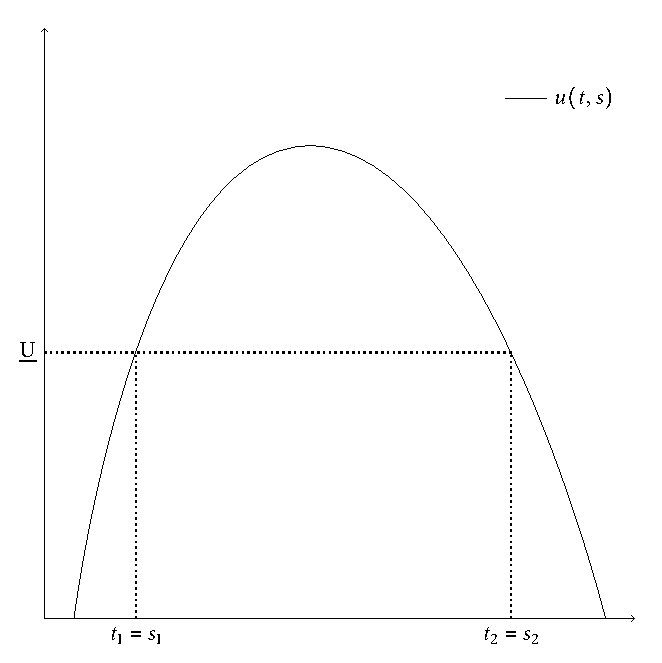
\includegraphics[width=0.75\textwidth]{acceptable-treatment.pdf}
	\caption{The patient minimum level of acceptable treatment given \(s\)}
	\label{fig:acceptable-treatment}
\end{figure}
% section the_patients_problem (end)
%%--------------------------------------------------------------------------
%% Section: The physician problem
%%--------------------------------------------------------------------------

\section{The physician problem}
%In this section I describe the physicians problem in more detail. An important assumption, is that while the physician cannot observe \(s\), he has an unbiased estimate of \(s\), in the sense that the mean of \(G(s\mid x)\) is equal to the true level of \(s\).

The physician has a utility function given by
\[
	V=v(M,\eta)
\]
where the physicians payment, \(M\) is given by
\[
	M=\delta+(p-\omega)t 
\]
where \(\delta\) is a fixed payment, \(p\) is the physician payment per unit of treatment, \(t\) is quantity of treatment.

 I also assume that the physician can increase the quality of treatment by increasing the diagnosis accuracy through effort, such that \(\eta\) increases proportionally to the effort applied. Thus \(\eta\) is the both level of accuracy in \(X^\eta\) and the physicians effort. 

 The cost of accuracy is given by a continues, increasing and convex cost function \(C\). Assuming a separable utility function, the physician problem can be expressed as
\[
	v(M,\eta)=M-C(\eta)
\]
As the subject of this paper, is the acquisition of information, through physician effort, I ignore the treatment decision and assume for simplicity that the payment for treatment \(p\) can be set exactly equal to the cost \(\omega\).  The problem then simplifies to
\begin{align}
v(\delta,\eta)=\delta-C(\eta)\label{eq:phys-utility}
\end{align}.

The physician will not apply effort, when the value function is negative. Therefor the maximum effort that he will apply is 
\[
	\delta=C(\eta)
\]
which implies that 
\[
	C^{-1}(\delta)=\eta
\]
is concave by the fact that the inverse of strictly increasing convex real function is concave.\footnote{
See \cref{sub:the_inverse_of_a_strictly_convex_function_is_concave} for a proof} Thereby the the limit of \(C^{-1}(\delta)\) exist and is given by 
\[
	\lim_{\delta \rightarrow\infty}C^{-1}(\delta)=\bar{\eta}
\]
Therefore it must be the case that \(\eta\in[0,\bar{\eta}]\) no matter the size of \(\delta\).
Further one might notice that a physician with higher cost of \(\eta\) will acquire less information than a physician with lower \(C\).  Taking the inverse and differentiating, I get  
\begin{align}
    (C^{-1})'(\delta)\delta'=1 \Leftrightarrow  (C^{-1})'(\delta)=\frac{1}{\delta'}\label{eq:cost-function}
\end{align}
notice that from the convexity of \(C\)  it follows that \(C_1>C_2 \Rightarrow C'_1>C_2'\), which again by \cref{eq:cost-function} implies that \((C^{-1}_1)'(\delta)<(C^{-1}_2)'(\delta)\). 

It is further assumed that the physician can store knowledge about patients, such that \(\eta(i)\geq\eta(j)\) for \(i>j\) always hold. 

\section{A static analysis} % (fold)
\label{sec:atatic_analysis}


% section atatic_analysis (end)
%%--------------------------------------------------------------------------
%% Section: The patients search for treatment in a static setting
%%--------------------------------------------------------------------------
\section{The patients search for the best treatment}

From \cref{eq:utility-increasing-information} it is clear that the patient will always prefer more information to less information. 

The patient is aware that she needs treatment, but the level of treatment is unknown. The patients does however know that physician will apply effort in the interval \([0,\sup\bar{\eta}]\). For simplicity I also assume that the patient is ignorant about the distribution of \(\eta\), such that \(\eta\sim \mathcal{U}(0,\sup\bar{\eta})\). The game is then as follows

\begin{enumerate}[label=\itshape Stage \arabic*:]
	\item Choose a random physician and get and expected utility of 
\begin{align}
    U(t,s;E\eta)=\int_{X}\int_{S}u(t,s)\dif G^{E\eta}(s\mid x)\dif F^{E\eta}(x)\label{eq:first-search}
\end{align},
	where \(E\eta\) is the expected value of \(\eta\)
	\item The patient observes the realization of \(t,\eta\). If the patient stays with the same physician she knows she gets a utility of \((U(t,s;\eta(i)))\), where \(\eta(i)=\Delta\eta(i)+\eta(j),\:i>j\). If she searches for another physician she will get \cref{eq:first-search}
	r
\end{enumerate}

The condition for staying is then 
\[
	U(t,s;\eta(i))>U(t,s;E\eta)
\]

%--------------------------------------------------------------------------
%% Dynamic Settings
%%--------------------------------------------------------------------------

\printbibliography

%%--------------------------------------------------------------------------
%% Appendix
%%--------------------------------------------------------------------------

%%--------------------------------------------------------------------------
%% Appendix
%%--------------------------------------------------------------------------

\begin{appendices}
\section{Appendix}\label{sec:appendix}
\subsection{More informative \& least as powerful test}\label{app:test-power}

See~\cref{fig:test-power}

\begin{figure}[!ht]
	\centering
	\begin{subfigure}[b]{\textwidth}
		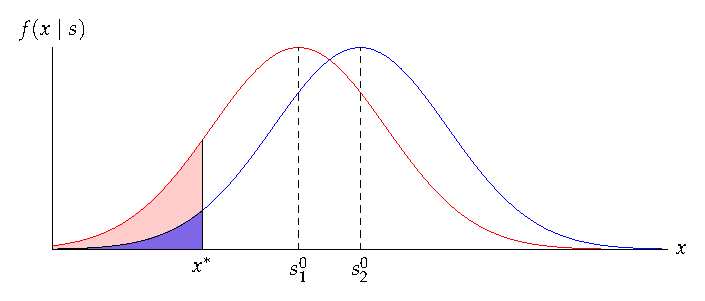
\includegraphics[width=\textwidth]{test-power-1.pdf}
		\caption{}\label{fig:test-power-1}
	\end{subfigure}
	\begin{subfigure}[b]{\textwidth}
		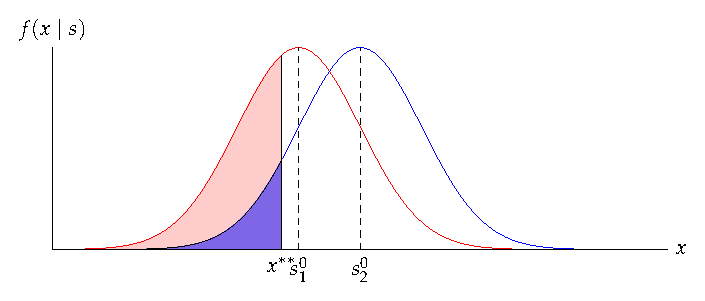
\includegraphics[width=\textwidth]{test-power-2.pdf}
		\caption{}\label{fig:test-power-2}
	\end{subfigure}
\caption{The blue shaded area is the probability of a type I error, and the red shaded area is the test power, while the non-shaded area under the red curve is the probability of a type II error. \Cref{fig:test-power-1,fig:test-power-2} have the same probability of a type I error, but the power of the test in \cref{fig:test-power-2} is higher than in \cref{fig:test-power-2}, as the probability of a type II error is smaller}\label{fig:test-power}
\end{figure}

%%--------------------------------------------------------------------------
%% Appendix: Stochastic Affiliation
%%--------------------------------------------------------------------------

\subsection{Stochastic Affiliation}\label{app:affiliation}
\begin{definition}
	The random variables $X_1,\ldots,X_n$ are said to be affiliated if their joint PDF $f(\mathbf{x})$ is log-supermodular, meaning that for  all $\mathbf{x},\mathbf{x}'\in\mathbb{R}_nb$, we have
	\[
		f(\mathbf{x}\land \mathbf{x}')f(\mathbf{x}\lor \mathbf{x}')\geq f(\mathbf{x})f(\mathbf{x}')
	\]
When $f$ is twice continuously differentiable, then equivalently $bX_1,\ldots,X_n$ are affiliated iff for all $i\ne j$
\[
	\frac{\partial^2}{\partial x_i \partial x_j}\ln f\geq 0
\]
\end{definition}
Consider two joint random variables $X$ and $S$. Affiliation then tells us about the conditional distribution of $f(S\mid x)$. If $x\leq x', y\leq y'$, then affiliation implies that
\[
	\frac{f(x,y')}{f(x,y)}\leq \frac{f(x',y')}{f(x',y)}
\]
which we can rewrite as
\[
	\frac{f(y'\mid x)f_X(x)}{f(y\mid x)f_X(x)}=\frac{f(y'\mid x)}{f(y\mid x)}\leq \frac{f(y'\mid x')}{f(y\mid x')} = \frac{f(y'\mid x')f_X(x')}{f(y\mid x')f_X(x')}
\]
which tells us the that likelihood ratio $f(\cdot\mid x)\big/ f(\cdot\mid x)$ is increasing in $x$ and thereby displays the monotone likelihood ratio property, which implies first-order (and hence second-order) stochastic dominance. \cite[in proposition 8 and 10 ]{Quah2009Comparative}, proofs that the monotone likelihood ratio property is required for the family of functions with the single-crossing property to have an increasing optimal solution in the signal $x$.

A further property of affiliation is that it is preserved under Bayesian updating, such that if the prior $f(s')\big/f(s),\, s'\geq s$ has a monotone likelihood ratio property, then the posterior $f(s'\mid x)\big/f(s\mid x)$ also have the monotone likelihood ratio property for any likelihood function $f(x\mid \cdot)$.

At last, affiliation is also preserved under multiplication, such that if $f(\mathbf{x})=h(\mathbf{x})g(\mathbf{x})$, where $g$ and $h$ is nonnegative and affiliated, then $f$ is also affiliated.
%%--------------------------------------------------------------------------
%% Appendix: Proof Topiks
%%--------------------------------------------------------------------------

\subsection[A simplified proof of Topkis’s Monotonicity Theorem is]{A simplified proof of \Citeauthor{Topkis1998Supermodularity}'s Monotonicity Theorem}\label{app:topiks-proof}
\begin{theorem}
	Consider the problem
	\[
		t^*(s)=\argmax_{s\in S} u(t,s)
	\]
	where $T,S\in \mathbb{R}$ and $T_s\subset T$ is the correspondence from $S$ to $T$  with $T_s$ being the set of feasible treatments, when the diseases is $s$.  Assume also that
	\begin{enumerate}[label=(\roman*)]
		\item $u$ has increasing differences in $(t,s)$  and
		\item $T_s=[g(s),h(s)]$  where $h,g:S \rightarrow \mathbb{R}$ are increasing functions with $g\leq h$
	\end{enumerate}
	Then the maximal and minimal selection of $t^*(s)$, $\bar{t}(s)$ and $\underbar{t}(s)$ is an increasing functions.
\end{theorem}

\begin{proof}
	The proof is done by contradiction. Assume that $\bar{t}(s)$ is not increasing. Then for some $s'>s$  $\bar{t}(s')<\bar{t}(s)$.  Then using assumption (ii) and the fact that $\bar{t}(s)\in T_s$  and $\bar{t}(s')\in T_{s'}$  it follows that $g(s)\leq g(s')\leq \bar{t}(s') < \bar{t}(s) \leq h(s) \leq h(s')$  so that $\bar{t}(s)\in T_{s'}$ and $\bar{t}(s')\in T_s$.  Using the latter facts along with $\bar{t}(s)\in t^*(s)$ and $\bar{t}(s')\in t^*(s')$  we have
	\begin{alignat*}{3}
	   & 0 && \geq u[s',\bar{t}(s)]-u[s',\bar{t}(s')] && \qquad \text{By optimality of } \bar{t}(s') \\
	   &   && \geq u[s,\bar{t}(s)]-u[s,\bar{t}(s')]   && \qquad \text{by increasing differences *} \\
	   &   && \geq 0                                  && \qquad \text{by optimality of } \bar{t}(s)
	\end{alignat*}
	which holds throughout. Hence it follows that $u(s',\bar{t}(s))=u(s',\bar{t}(s'))$, such that $\bar{t}(s)\in t^*(s')$, which is a contradiction to the fact that $\bar{t}(s')=\max \{t^*(s')\}$ in the view of $\bar{t}(s')<\bar{t}(s)$.  Hence, $\bar{t}(s)$ is an increasing function. The proff for $\underbar{t}(s)$ is symmetric \parencite{Amir2005Supermodularity}.\footnote{In this proof, it is assumed that $T_s\cap T_{s'}\ne \emptyset$. If this was the case, one would have that $\sup T_s < \inf T_{s'}$ and it follows trivially have that $t^*(s)<t^*(s')$}
\end{proof}
\subsection{The inverse of a strictly convex function is concave} % (fold)
\label{sub:the_inverse_of_a_strictly_convex_function_is_concave}
\begin{theorem}
Let $f$ be a real function which is convex on the open interval $I$, and let $J=f(I)$. Then if $f$ is strictly increasing on $I$, then $f^{-1}$ is concave on $J$.
\end{theorem}
 \begin{proof}
 Let $X=f(x)\in J$ and $Y=f(y)\in J$. From the definition of a convexity, it follows that $\forall a,b\in \mathbb{R}_{++}, a+b=1:f(ax+by)\leq af(x)+bf(y)$. 

Let $f$ be increasing on $I$. Then $f^{-1}$ is increasing on $J$, as the inverse of a monotone increasing function is increasing. Thus, $af^{-1}(X)+bf^{-1}(Y)=ax+by\leq f^{-1}(aX+bY)$, and hence $f^{-1}$ is concave on $J$
 \end{proof}
% subsection the_inverse_of_a_strictly_convex_function_is_concave (end)


\end{appendices}
